\documentclass[../report.tex]{subfiles}
 
	The primary intent of the project is to be able to use the data generated by the \textit{SAX} algorithm to detect events in a measurement over a period of time.  One existing common technique for doing this is STA/LTA (Short Term Average/Long Term Average) \citep{man-seis-obs}.  STA/LTA is a sliding window technique where the mean of the absolute amplitudes are compared ofver two different sized windows.  If the STA exceeds the LTA by a preset threshold then an event is triggered, if it drops below another threshold the trigger is ended.  The event is considered the duration between these two triggers.
	
	In order to evaluate a SAX based detection algorithm, an implementation of STA/LTA was required for comparison  Traditionally STA/LTA thresholds are set manually by experienced seismologists, in this case however, the author does not have the required experience to set these values so an adaptive method was required.
	
\subsection{Adaptive STA/LTA Algorithm} \label{sec:stalta-detect}
	\textit{N.B.  This implementation has only been validated on a relatively small sample set and is not recommended for real-world use without further testing.}

	The algorithm works by iterating through the data on two sliding windows calculating a short and long term mean of the absolute values of the amplitude.

	\noindent
	\\
	$l = $ number of datapoints in LTA \\
	$s = $ number of datapoints in STA \\

\begin{equation}
	\overline{LTA} = \sum_{i=1}^{l}\dfrac{\abs{v(t - i)}}{l}
\end{equation}

\begin{equation}
	\overline{STA} = \sum_{i=1}^{s}\dfrac{\abs{v(t - i)}}{s}
\end{equation}
	
	For each iteration, the STA is compared to a number of standard deviations (typically 3) from the LTA, if it exceeds this value, the event is considered triggered on.  The current value of the LTA is then stored.
	
	The iteration then continues calculating STA with the triggered value set to true until the STA drops below the original LTA value when the event was triggered.
	
	If the event duration is above a pre-set threshold (typically 5s) then the event is recorded, if not the it is discarded as a probable spike.	

	One downside to this approach is that it cannot normally detect an event within the period of the LTA from the start of the observation window.  It also struggles to detect an event when there is significant background noise.
	
\subsection{SAX Detection Algorithm} \label{sec:sax-detect}

	The \textit{SAX Detection Algorithm} works by firstly calculating a SAX string for the whole observation.  It requires a minimum \textit{trigger on} length in milliseconds (to eliminate spikes), a quiet duration (again in milliseconds) and a distance from the centre value of the alphabet used to produce the SAX string.  This string is then iterated over one character at a time filling a ring buffer that is at least the length of the \textit{trigger on} or the \textit{quiet duration} that is used to establish whether trigger requirements are met.  It is effectively an implementation of Step Detection using the breakpoints defined in the SAX process.
	
	\lstinputlisting[language=Python]{../seismic/detector/sax.py}

% Discuss 

\subsection{Approximate Detection of Events by Distribution}

	Following on from the discussion in \cref{sec:distribution} and based on a hypothesis that background noise is effectively random and with a high enough number of samples would follow the Central Limit Theorum, it follows that only when a sample contains both background noise and an event would its normalised distribution deviate significantly from a normal one.
	
	By applying the SAX algorithm to a sample of data, it has effectively been bucketed against a normal or Gaussian distribution.  It therefore leads that the distribution of counts of each symbol in the sample provide an approximate measure of how close the sample is to being normally distributed.
	
	A function was written to sample a window of length \textit{w}, perform PAA and SAX on it and calculate the standard deviation normalised by the number of samples over the number of symbols.  The window is then shifted to the right by $\frac{w}{2}$ places run again.  This is repeated for the whole observation.  The effectiveness of this method is shown in \cref{fig:disttest}.  The top plot shows a raw trace over a 24 hour period for the station YW.NAB1 at the Nabro Volcano in Eritrea on 2011-08-27 \citep{eritrea1} and the bottom plot shows the aforementioned sliding window SAX distribution function with a \textit{w} of 300s, a PAA interval of 50ms and an alphabet of length 7 with a trigger value set to 0.25.
	
	It can be seen from the two plots imposed next to each other that the spikes from the SAX distribution function correlate almost perfectly with the visible events on the trace, albeit at a much lower resolution (2.5 minutes as opposed to 0.1 seconds in this case).
	
\begin{figure}[H]
	\centering
	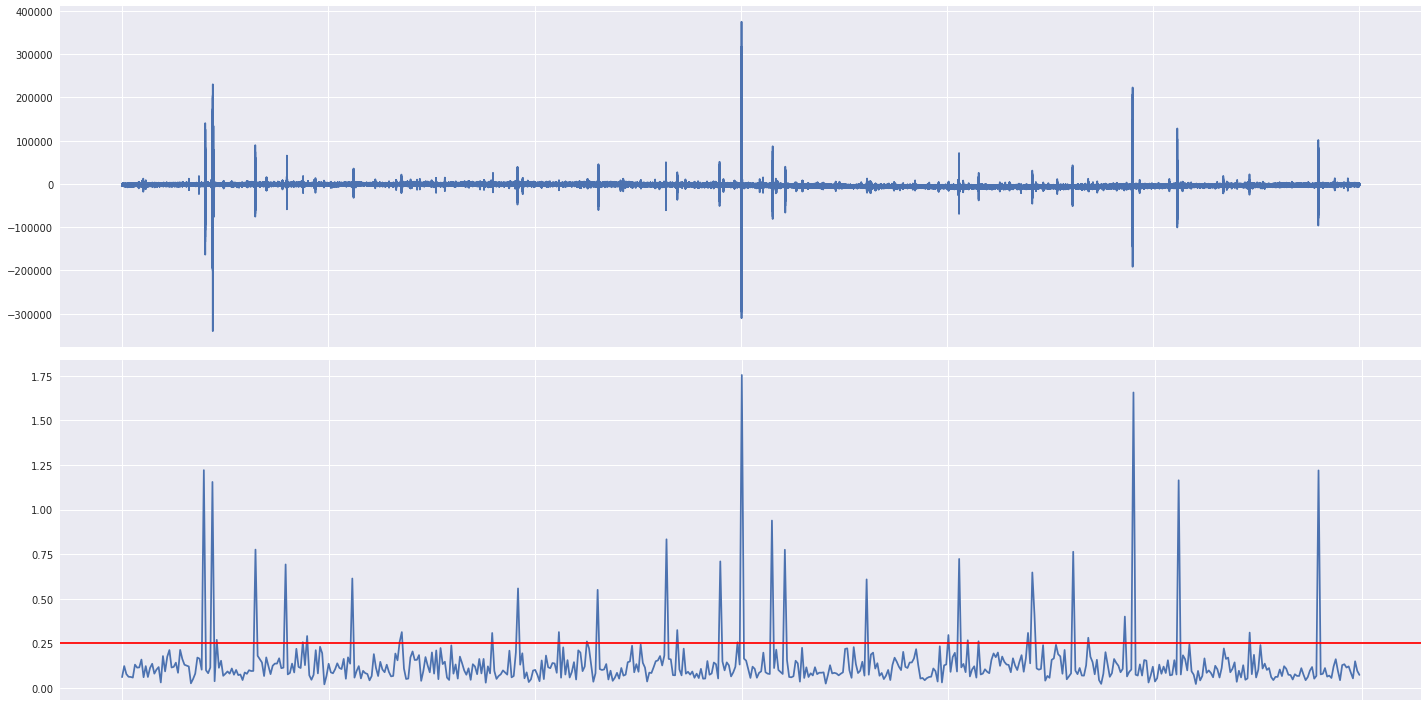
\includegraphics[width=1\linewidth]{img/dist_test}
	\caption{Using SAX distribution for approximate event finding}
	\label{fig:disttest}
\end{figure}

\subsection{Combining the Approximate Detection with the SAX detection}

	The SAX distribution approximation function returns probable events in a 5 minute window.  These windows can then be passed to the SAX Detection Algorithm described in \cref{sec:sax-detect} which has been shown to be effective over shorter windows.  Computationally, the combined process takes approximately 10 seconds to run over a 24 hour period with a sampling rate of 100Hz one an Intel(R) Xeon(R) CPU E3-1505M v5 @ 2.80GHz once the whole observation is loaded in to memory as a Pandas Series object.  Although by the nature of Python's threading model it cannot be optimised for multiple cores for a single observation, there is no reason why it cannot be run in parallel against multiple observations.  This is the model that the worker process described in \cref{sec:worker} takes.